\section{LTCC Refurbishment}


The re-scoping of the LTCC to discriminate pions instead of electrons required a dramatic increase in the
number of photo-electrons detected. Four areas were considered to achieve this:

\begin{enumerate}
	\item Increase optical reflectivity
	\item Increase PMT response to UV light
	\item Increase gas volume
	\item Address the gas leaks and other hardware issues.
\end{enumerate}


Monte-Carlo simulations of pions in the LTCC quantified the number of Cherenkov light  reflections on the cylindrical, elliptical,
parabolic and Winston cones surfaces as:

\begin{itemize}
	\item 2 reflections only: $30\%$ of the time
	\item 3 reflections: $40\%$ of the time
	\item 4 or more reflections: $30\%$ of the time
\end{itemize}

These results were confirmed with empirical observations during the mirror aligmnent.

A study of refurbishment of the mirror and Winston cone surfaces
involved re-coating samples of surfaces and mirrors using several companies.
The original average measured reflectivity of the mirrors and Winston cones
showed a degraded reflectivity compared to the values at installation and to
the new samples, probably due to  17 years of aging, see \F{reflectivityGain}.


\begin{figure}
	\centering
	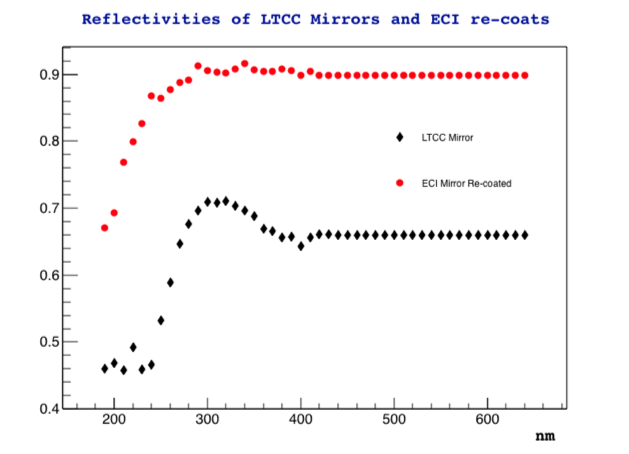
\includegraphics[width=1.0\columnwidth,keepaspectratio]{img/reflectivityGain.png}
	\caption{A typical reflectivity measurement of one original LTCC mirror (black diamond) shows a 65\% reflectivity versus what can be achieved
		      by a new coating (red dots), about 90\% reflectivity. The increase is even more significant at smaller wavelengths }
	\label{fig:reflectivityGain}
\end{figure}

In the study a few scenarios using the $C_4F_{10}$ index of refraction (shown in \F{c4f10RefrIndex})
and considering the various reflection probabilities outlined above  were considered:

\begin{figure}
	\centering
	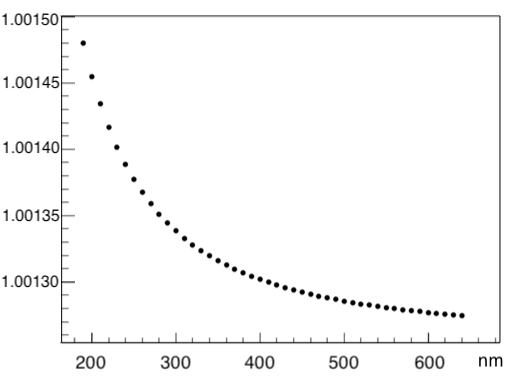
\includegraphics[width=1.0\columnwidth,keepaspectratio]{img/c4f10RefrIndex.png}
	\caption{The $C_4F_{10}$ gas refraction index as a function of wavelength.}
	\label{fig:c4f10RefrIndex}
\end{figure}

\begin{itemize}
	\item using old or new mirror reflectivity (see \F{reflectivityGain})
	\item using a completely transparent gas or the $C_4F_{10}$ with its measured transparency
	\item using the actual or the enhanced PMT quantum efficiency function
	\item using or not the additional $C_4F_{10}$ gas volume
	\item comparing the pion response to the original CLAS 6 GeV era electron response
\end{itemize}

The distributions for each scenario were plugged in the Frank\textendash Tamm formula \cite{Frank:1937fk} below to calculate
the Cherenkov radiation yield as a function of wavelengh and momenta:

%~\ref{eq:cerenkov}.

\begin{equation} \label{eq:cerenkov}
	\frac{d^2n}{dxd\lambda} = \frac{2\pi z^2\alpha}{\lambda^2}\sin^2{\theta_C(v)},
\end{equation}

where $\alpha$ is the fine structure constant and $\theta_C$ is the \u{C}erenkov cone half-angle.

One particular combination among the described scenarios is given as an example \F{photonYieldStudy} for pions,
the measured unfurbished mirror reflectivity, a $100\%$ transparent gas and a PMT with ideal refusrbished quantum efficiency.

\begin{figure}
	\centering
	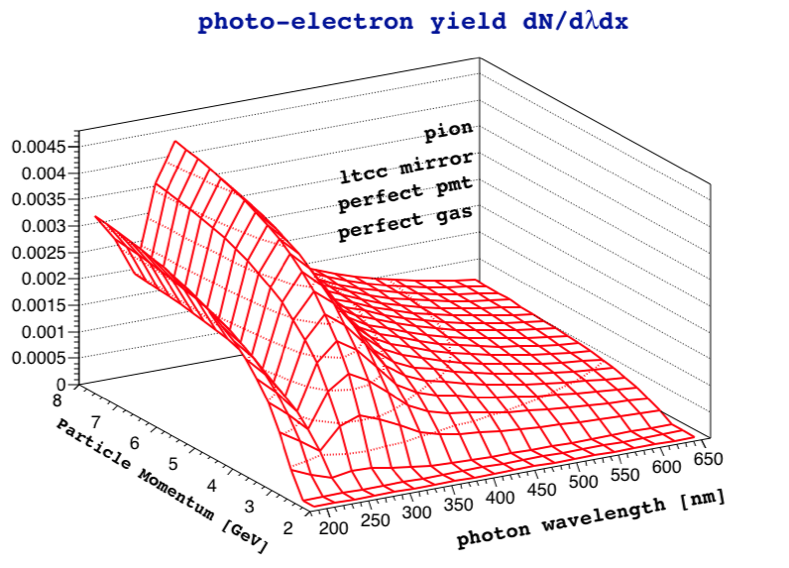
\includegraphics[width=0.95\columnwidth,keepaspectratio]{img/photonYieldStudy.png}
	\caption{Cherenkov light yield as a function of pion momentum and photon wavelength using the Frank\textendash Tamm for one of the scenarios considered:
            mirrors and Winston cones with low reflectivity (ltcc original mirror, not refurbished), a perfectly transparent gas and an ideally refurbished PMT.}
	\label{fig:photonYieldStudy}
\end{figure}


When the number of reflections is taken into account, the refurbishment shows
a factor of 2.4 gain in the visible light wavelengths and a factor of 3 in the UV:

%\begin{itemize}
%	\item Visible:
%	\begin{itemize}
%		\item original integrated reflectivity: $27.5\%$ (1 reflection $65\%$)
%		\item refurbished integrated reflectivity: $68.1\%$  (1 reflection $88\%$ )
%	\end{itemize}
%	\item Ultra violet:
%	\begin{itemize}
%		\item original integrated reflectivity: $9.1\%$ (1 reflection $45\%$)
%		\item refurbished integrated reflectivity: $34.3\%$  (1 reflection $75\%$ )
%	\end{itemize}
%\end{itemize}

\begin{itemize}
	\item Visible:
	\begin{itemize}
		\item original integrated reflectivity: $27.5\%$
		\item refurbished integrated reflectivity: $68.1\%$
	\end{itemize}
	\item Ultra-violet:
	\begin{itemize}
		\item original integrated reflectivity: $9.1\%$
		\item refurbished integrated reflectivity: $34.3\%$
	\end{itemize}
\end{itemize}


The results have been summarized in \F{refurbishmentGains} for two main scenarios: mirror re-coating and PMT quantum efficiency improvements.
By performing both of these improvements the study shows that the LTCC response to pions will be the same as it was for electrons above 4 GeV.

\begin{figure}
	\centering
	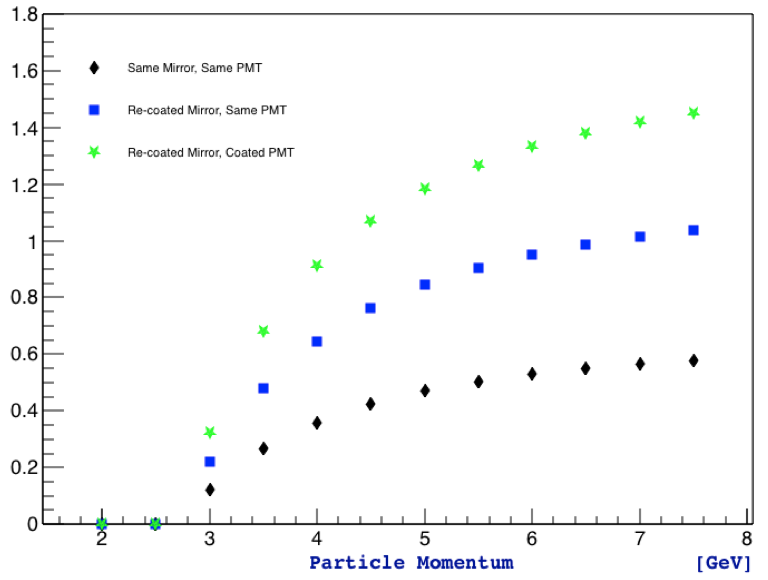
\includegraphics[width=0.95\columnwidth,keepaspectratio]{img/refurbishmentGains.png}
	\caption{Ratio of LTCC response to pions to old response to electrons. Black diamonds: with no refurbishment, the goal of detecting pions cannot be reached.
            More than a factor of two can be gained by recoating the mirrors and Winston cones (blue squares). In addition, by increasing the
            PMT response to UV light (green stars), the LTCC can reach the old performance above pion momenta of 4 GeV.}
	\label{fig:refurbishmentGains}
\end{figure}

The design changes of the LTCC are summarized below:

\begin{enumerate}
\item Resize the box to fit in the reduced space between the Drift Chambers and the Forward Time-Of-Flight:
	\begin{enumerate}
		\item Cut Sides
		\item Relocate the three mirror sets closest to the back-wall
		\item Redesign, replace back-wall frame
	\end{enumerate}

	\item Decrease inefficient regions
	\item Increase PMT gain, split output to provide both FADC and TDC signals
	\item Minimize gas leaks
	\item Better mirror supports
	\item Increase light yield:
	\begin{enumerate}
		\item Re-coat all mirrors
		\item Re-coat Winston Cones
		\item Wavelength shifting re-coating of the PMTs
		\item Add nose to increase gas volume
	\end{enumerate}
\end{enumerate}

\subsection{Box Modifications}





\paragraph{Box Cut}
\paragraph{Nose}
\paragraph{Mirrors re-location}
\paragraph{Back-wall}
\paragraph{Connectors}
\paragraph{Mirror Support}



- Use Hermetical signals, HV connectors
- Seal the box from the inside
- Window: glue + sealant

\subsection{Mirror re-coating}

As seen in \F{optics}, each LTCC segment is composed of four optical surfaces: one elliptical mirror,
one hyperbolic mirror, one cylindrical mirror, and the Winston cone.
The reflectivity of a random selection of 30 elliptical, cylindrical, and hyperbolic mirrors from two sectors was measured.
All the mirrors analyzed showed significant degradation from the original desired reflectivity of 90$\%$ in the visible spectrum,
see for example \F{reflectivityBeforeAndAfter} (top).
A refurbishment of the mirrors was crucial to enhance the detector response to the emitted pion Cherenkov light.
Due to the material, assembly, and dimensions of the different types of mirrors, two different techniques were employed to refurbish the
reflective surfaces as discussed below.

\begin{figure}
\centering
	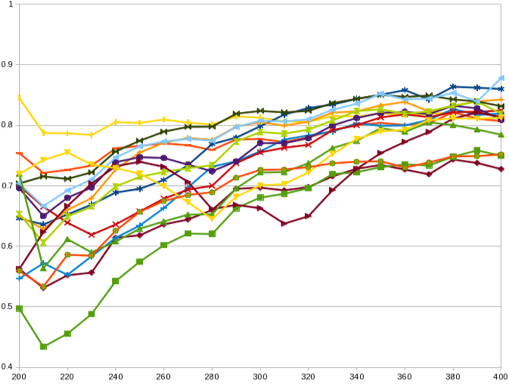
\includegraphics[width=0.99\columnwidth, height=0.7\columnwidth]{img/mirrorsReflectivityBefore.png}
	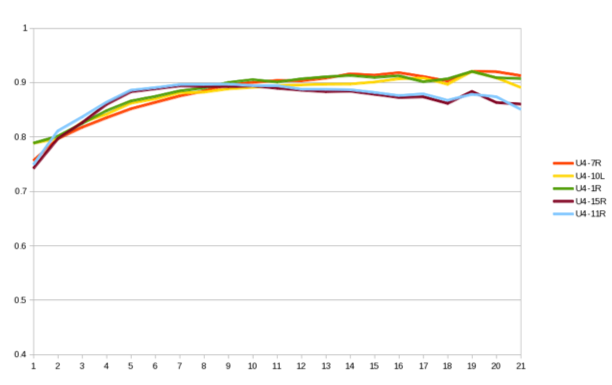
\includegraphics[width=0.99\columnwidth, height=0.7\columnwidth]{img/mirrorsReflectivityAfter.png}
	\caption{Top: Reflectivity measurement as a a function of wavelength of a sample of 8 mirrors before re-coating,
            each sampled at two different places on their surface. The reflectivity
			was measured using a monochromator (Newport model CS260-USB-1-FH-A) with a deuterium light source with a reach
            between 200 nm and 400 nm. The average reflectivity was about 65$\%$ instead of an optimal 90$\%$.
			Bottom: Reflectivity measurement as a function of wavelength of a sample of 5 mirrors measured
            after gluing on the Lexan strips (see text for detail).
            Note the very high value of reflectivity in the UV region, where most of the Cherenkov light is produced.
            In the visible spectrum, the reflectivity is about 90$\%$.}
	\label{fig:reflectivityBeforeAndAfter}
\end{figure}


\subsubsection{Re-coating of cylindrical mirrors}

The cylindrical mirrors range from 6 to 12 inches in length. Each mirror is made from a single piece of aluminum or plastic.
Due to their small size, they fit in most vacuum chambers used to coat mirrors by evaporation of aluminum with magnesium fluoride
(AlMgF$_2$). After successful testing of re-coating of AlMgF$_2$ onto the existing substrate, the work of re-coating the 216 cylindrical mirrors
was awarded to ECI~\cite{ECI}. See \F{reflectivityBeforeAndAfter} (bottom) for typical reflectivity values after re-coating.

\subsubsection{Re-coating of elliptical and hyperbolic mirrors}

The elliptical and hyperbolic mirrors are composed of a Kevlar support structure with a Lexan substrate.
It was not possible to changed this hardware from its original design and construction in 1997.
The support material, which allowed for pitch, roll, and yaw alignment of the mirrors, included
wood and aluminum that was glued to the support structure.

Several companies attempted to re-coat these mirrors but failed due to the outgassing of the various materials.
Furthermore, many of the mirrors are $>$1 m in length, longer than most vacuum chambers.
Therefore the AlMgF$_2$ could not be re-deposited directly onto the mirror substrates.

A different approach consisted of coating thin (25 $\mu$m) Lexan strips and gluing the strips onto the mirror substrate.
While promising, this presented the challenge of protecting the coated Lexan strip from shipping and handling and
from the gluing procedure to the mirrors.

A working chain was setup to:

\begin{enumerate}
	\item coat the Lexan strip
	\item protect the strip with a temporary peel-able film for shipping and handling
	\item ship to Jefferson Lab
	\item glue the strip to mirror substrates
	\item remove the protective film
	\item test the reflectivity
\end{enumerate}

An example of unwrapping the film off the Lexan strip is shown in \F{filmOnStrip}. Several companies produced various test samples with
various protective material films. The job was eventually awarded to ECI \cite{ECI}.
The gluing of the strips to the mirror was done at Jefferson Lab. The mirrors were vacuum-holded on a supporting structure.
Loctite spray contact adhesive glue was applied on the mirror and directed out by a venting system.
The strip was applied to the substrate and after 24 hours of curing time the film was removed.
The typical reflectivity of the refurbished mirrors is shown in \F{reflectivityBeforeAndAfter} (bottom).


\begin{figure}
\centering
	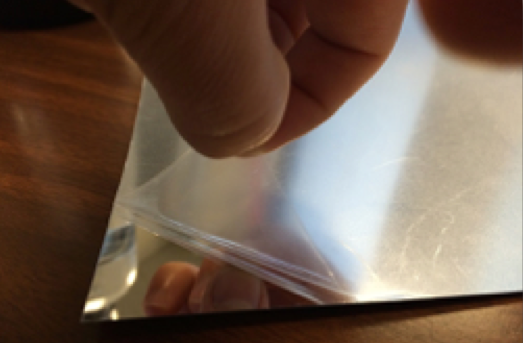
\includegraphics[width=0.98\columnwidth, height=0.7\columnwidth]{img/filmOnStrip.png}
%	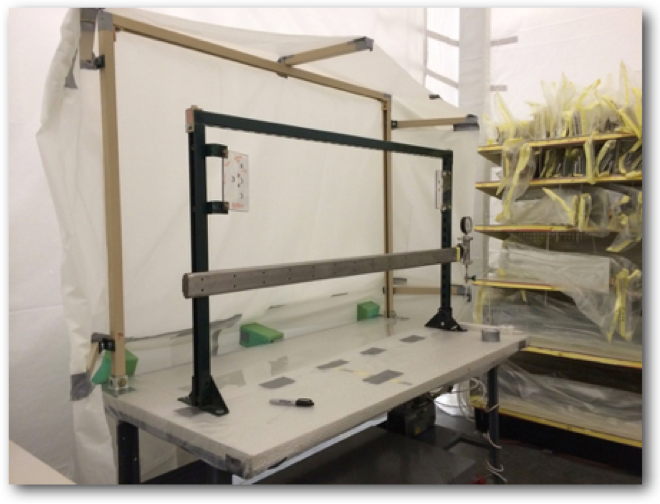
\includegraphics[width=0.98\columnwidth,keepaspectratio]{img/mirrorSetup.png}
	\caption{The protective film. For the elliptical and hyperbolic mirrors the Lexan strips were coated with AlMgF$_2$
			 and covered with films to protect the mirrors during handling and the gluing on top of the mirror substrates.
             The photograph shows the process of removing the protecting film from one such strip.
             The surface reflectivity was tested immediately after the installation on the substrate and again 48 hours after that.
             Only the samples from ECI \cite{ECI} resulted in a consistent high reflectivity. }
	\label{fig:filmOnStrip}
\end{figure}


\subsubsection{Elliptical mirror gaps}

The LTCC elliptical mirrors, especilly the longest ones, presented several gaps between the mirrors, some a few cm long.
This was evident also in the data analyses as a loss of efficiency between the mirrors.
To make sure that no light is lost in these gaps, additional 120 $\mu$m thick Lexan extension strips were produced and coated with AlMgF$_2$.
These strips were manufactured by ECI~\cite{ECI}. They were fitted and glued on left side elliptical mirrors to cover the gaps,
see \F{gapBeforeAndAfter}.

\begin{figure}
\centering
	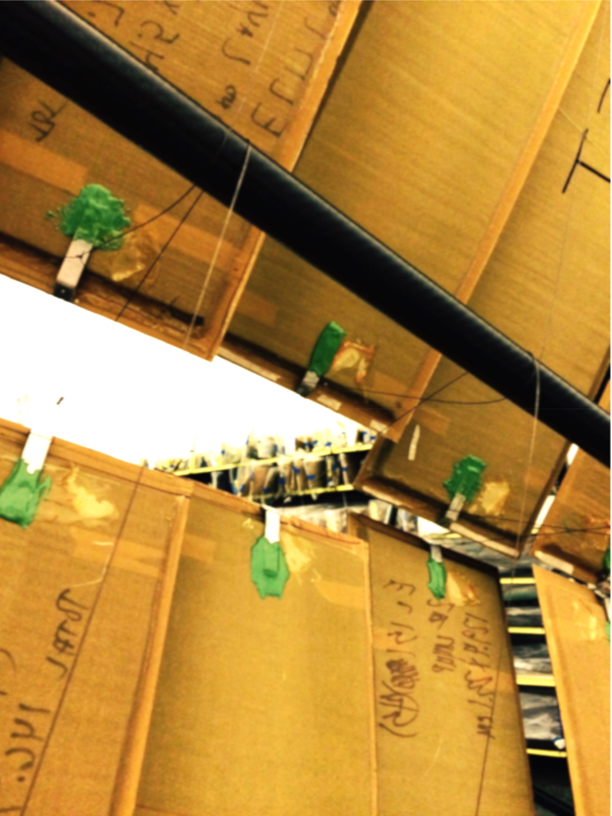
\includegraphics[width=0.98\columnwidth, height=0.7\columnwidth]{img/gapBefore.png}
	\includegraphics[width=0.98\columnwidth, height=0.7\columnwidth]{img/gapAfter.png}
	\caption{Top: the gaps between mirrors before refurbishing LTCC. These gaps were also seeing in the data as
			 drop of efficiency near the middle of the detector, as the Cherenkov light was not collected.
             Bottom: all the gaps are covered by the extension strips.}
	\label{fig:gapBeforeAndAfter}
\end{figure}


\subsubsection{Mirror re-coating summary and results}

All 216 cylindrical mirrors were re-coated on the existing surface. All 216 elliptical and 216 hyperbolic mirrors were refurbished using Lexan strips
coated with AlMgF$_2$ glued onto the substrate. The different sizes of the mirrors were accounted for using different widths for the Lexan strips, see
summary Table~\ref{tab:strips}.


\begin{table}
	\begin{center}
		\begin{tabular}{| l | c |}
			\hline \hline
			Quantity  & Dimensions (inches) \\
			\hline
			190       & 9  x 36 x 0.010  \\
			150       & 10 x 36 x 0.010  \\
			6         & 10 x 36 x 0.010  \\
			\hline \hline
		\end{tabular}
	\end{center}
	\caption{Summary of material used for the elliptical and hyperbolic mirrors. The total length of the Lexan strip necessary to re-coat the 216 elliptical
            and 216 hyperbolic mirror was 310 meters.}\label{tab:strips}
\end{table}


In \F{reflectivityBeforeAndAfter} (bottom) a typical spectrum of reflectivity that applies to all cylindrical, elliptical, and hyperbolic mirrors is shown.
The re-coated mirrors show a $\sim 90\%$ reflectivity in the visible spectrum and an exceptional $\sim 80\%$
reflectivity in the UV spectrum.



\subsection{Mirror alignment}

A new procedure was developed to align the mirrors within the LTCC boxes that takes advantage of their focusing capabilities.
The elliptical mirror focal points (see \F{alignmentSimulation}) are 1. the target (origin of the lab coordinate system)
and 2. a point behind the hyperbolic mirror. The focal points of the hyperbolic mirrors are 1. a point near the focal point of the elliptical mirrors and
2. a point above the face of the PMTs.

The geometrical shape of the mirrors has been built into the CLAS12 Geant4 simulation \cite{gemc2019}.
When a laser line coming from the target is directed at the mirror,
it is focused on the hyperbolic focal point, then directed at the PMT, see \F{alignmentSimulation}.
This geometrical focusing was used during the mirror alignment: a 3 mW, 635 nm laser was placed, relative to the detector,
in center of the CLAS12 coordinate system, the location of the liquid-hydrogen target and the first ellipse focal point.
The laser was mounted on a structure that allowed the beam direction and line angle to move with respect to the floor, while keeping
the origin of the laser at the coordinate system origin.
This position was accurate at the 0.5 mm level. The laser was spread through two cylindrical lenses into a laser line and shone
longitudinally along the center-line of each elliptical mirror. Both the elliptical and hyperbolic mirrors were then
adjusted in pitch, roll, and yaw to minimize the light spot dimensions and to center it in the middle of the face of the PMT.
The PMT entry glasses were protected from the laser line with custom-fitted cardboard pieces. After alignment, the spot size of the laser was 5 mm.


\begin{figure}
\centering
	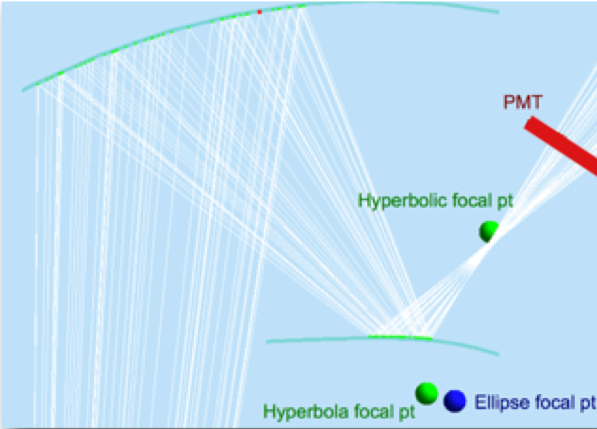
\includegraphics[width=0.99\columnwidth,  height=0.75\columnwidth]{img/mirrorAlignmentSimulationZoomed.png}
	\caption{The simulation of a laser line (white tracks are photons) originating from the target (first ellipse focal point) and directed at the elliptical mirrors.
             The photons are reflected to the second ellipse focal point. The hyperbole first focal point is near the ellipse focal point so the hyperbolic mirror
			 reflects the incoming photons to the hyperbole second focal point, located above the face of the PMTs.
			 This picture illustrates the procedure used for the alignment: the mirror positions are adjusted until the laser line originating from
			 the target is focused on the face of the PMT.}
	\label{fig:alignmentSimulation}
\end{figure}


%\begin{figure}
%\centering
%	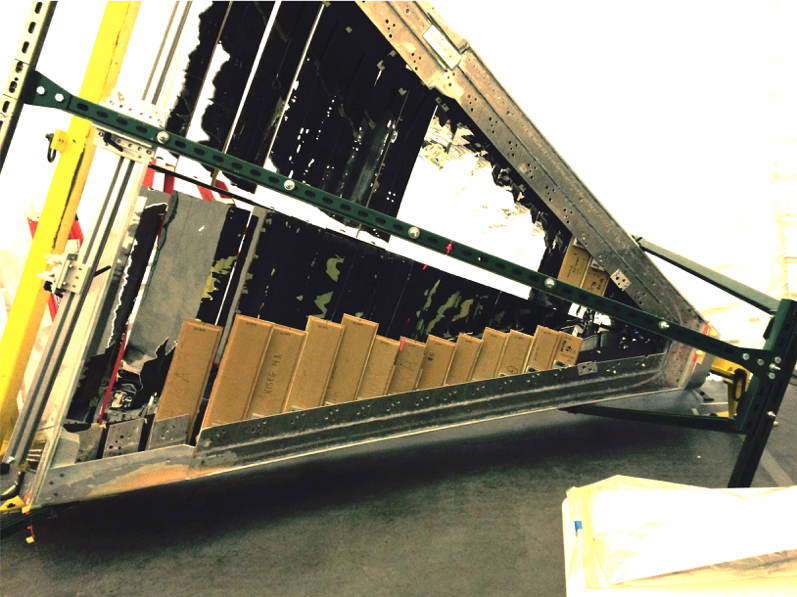
\includegraphics[width=0.95\columnwidth, keepaspectratio]{img/laserAlignment1.png}
%	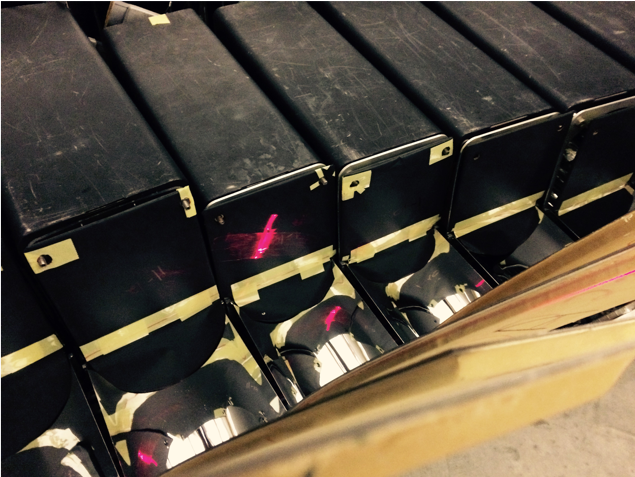
\includegraphics[width=0.95\columnwidth, keepaspectratio]{img/laserAlignment2.png}
%	\caption{The laser alignment setup. Top: the laser was placed, relative to the detector, in the lab coordinate system. The laser line was shined on each elliptical mirror.
%         Bottom: zoomed in view of the laser line focused on the center of the PMT after the mirrors were aligned.}
%	\label{fig:laserAlignment}
%\end{figure}


\subsection{Winston cone refurbishment}

Winston cones (WC) are used to collect light onto the PMTs. In the LTCC there are three kind of WCs:

\begin{enumerate}

\item Small
	\begin{enumerate}
		\item Height: 18 cm
		\item Radius at the top: 20 cm
		\item Radius at the bottom: 11 cm
		\item Material: 0.25 cm thick copper (electro-formed)
	\end{enumerate}

	\item Medium
	\begin{enumerate}
		\item Height: 22 cm
		\item Radius at the top: 20 cm
		\item Radius at the bottom: 11 cm
		\item Material: 0.5 cm thick plastic (vacuum pressed)
	\end{enumerate}

	\item Large
	\begin{enumerate}
		\item Height: 30 cm
		\item Radius at the top: 22 cm
		\item Radius at the bottom: 11 cm
		\item Material: 0.25 cm thick copper (electro-formed)
	\end{enumerate}
\end{enumerate}

\begin{figure}
	\centering
	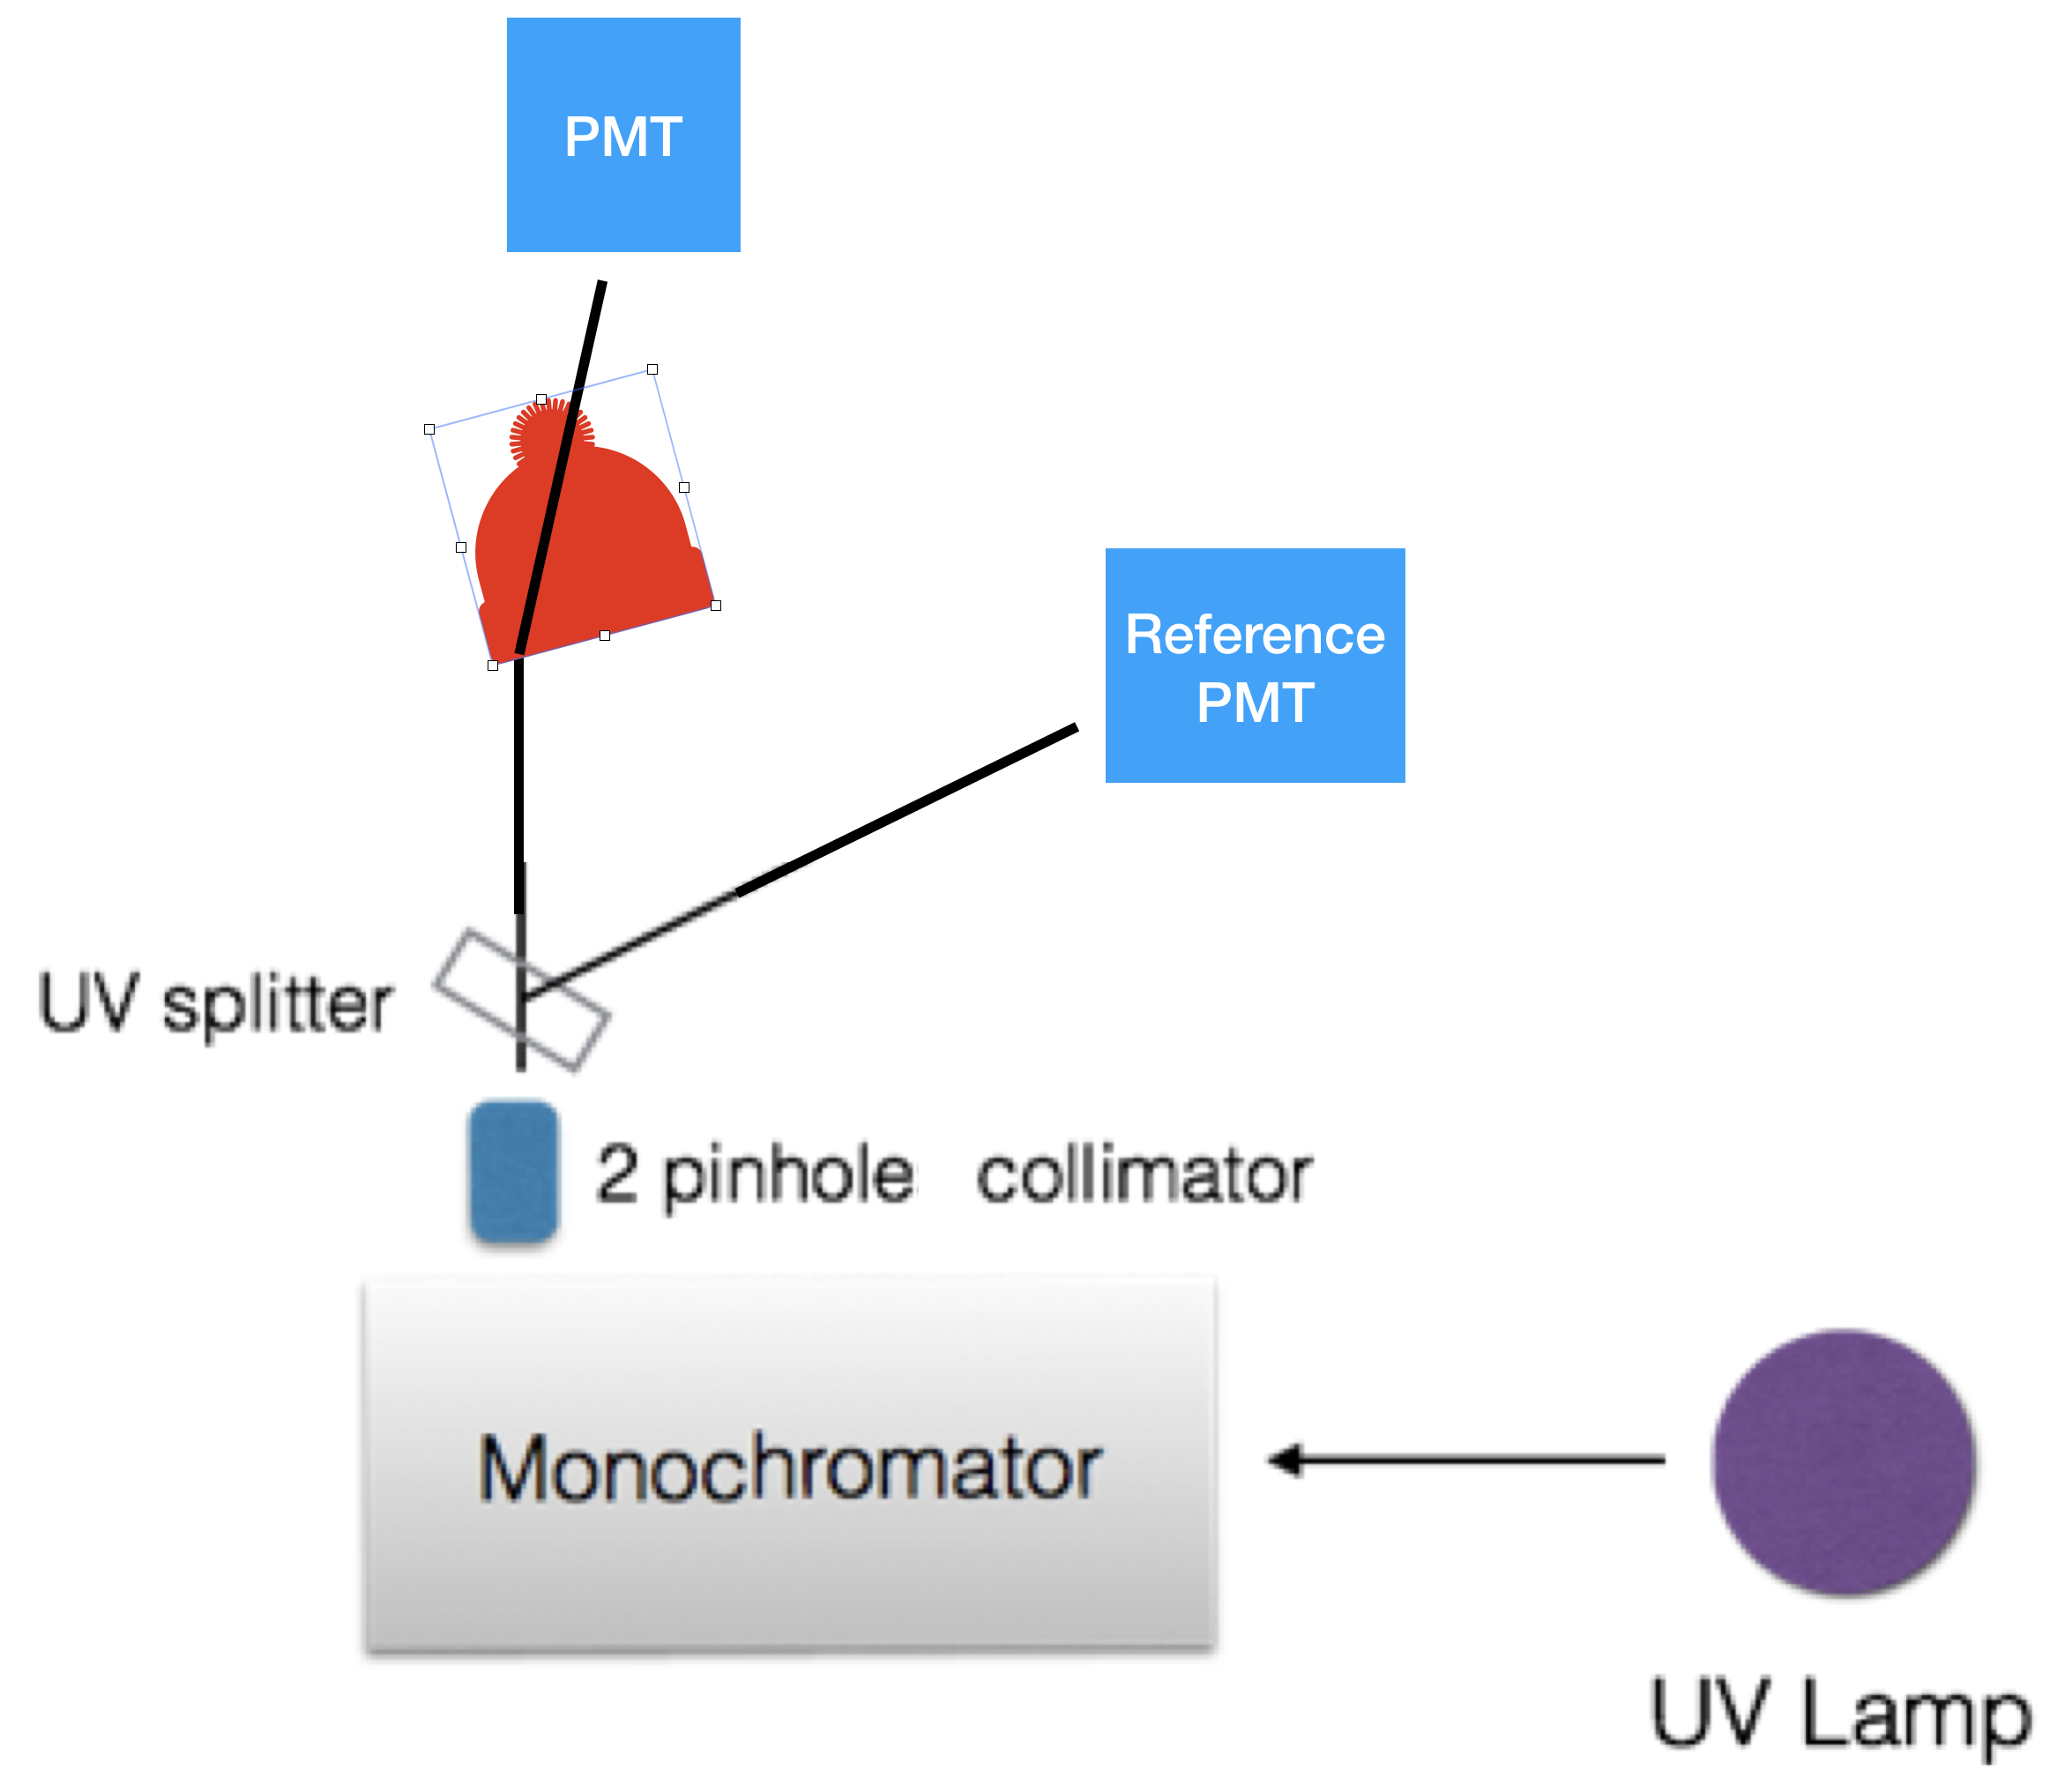
\includegraphics[width=0.95\columnwidth,keepaspectratio]{img/wcSetup.png}
	\caption{Setup to measure the WC reflectivity. The wavelength of light from a deuterium lamp was measured using a mono-chromator and splitted in two
            light beams, each with calibrated intensity. One of the light beam impinged on the WC at a typical angle of 12 degrees,
            while the other was directed at the reference PMT. }
	\label{fig:wcSetup}
\end{figure}

The reflectivity of the WC showed the same degradation as the mirrors. However, due to their shape, re-coating of the WC is more costly than the mirrors and the budget allowed
refurbishing of only 160 out of 216 total WCs.
A setup on an optical bench to measure the reflectivity for all the cones at wavelengths between 200 and 400 nm was designed to accept incident
shallow angles of 10-15 degrees (typical incidence angle based on simulation studies), see \F{wcSetup}. A typical reflectivity of a poor WC is shown in \F{wcStatusBefore} (top).
All 216 WC were measured, and the results are shown in \F{wcStatusBefore} (top). This allowed cataloging ofthe quality of the WC to select the worst ones to refurbish,
see \F{wcStatusBefore} (bottom).
The cones were put in a vacuum chamber and $AlMgF_2$ was deposited on top of the existing coating. The typical reflectivity of WC after recoating is shown in \F{wcStatusAfter} (top).
About 30 cones needed the additional treatment of removing the existing aluminum coating to improve the new $AlMgF_2$ deposition. Even then, about half of these cones did not show improvements.
The results of the WCs refurbishment are summarized in \F{wcStatusAfter} (bottom).


\begin{figure}
	\centering
	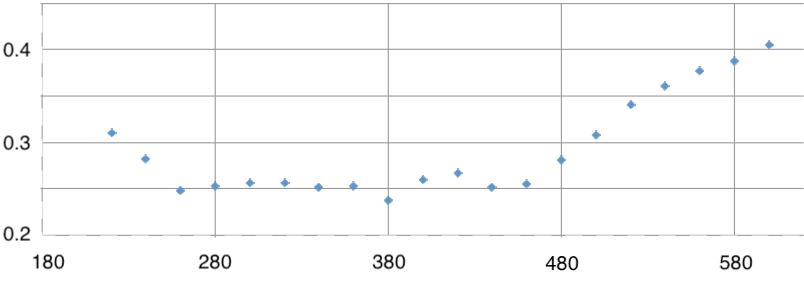
\includegraphics[width=0.95\columnwidth,keepaspectratio]{img/winstoConeSample2Reflectivity.png}
	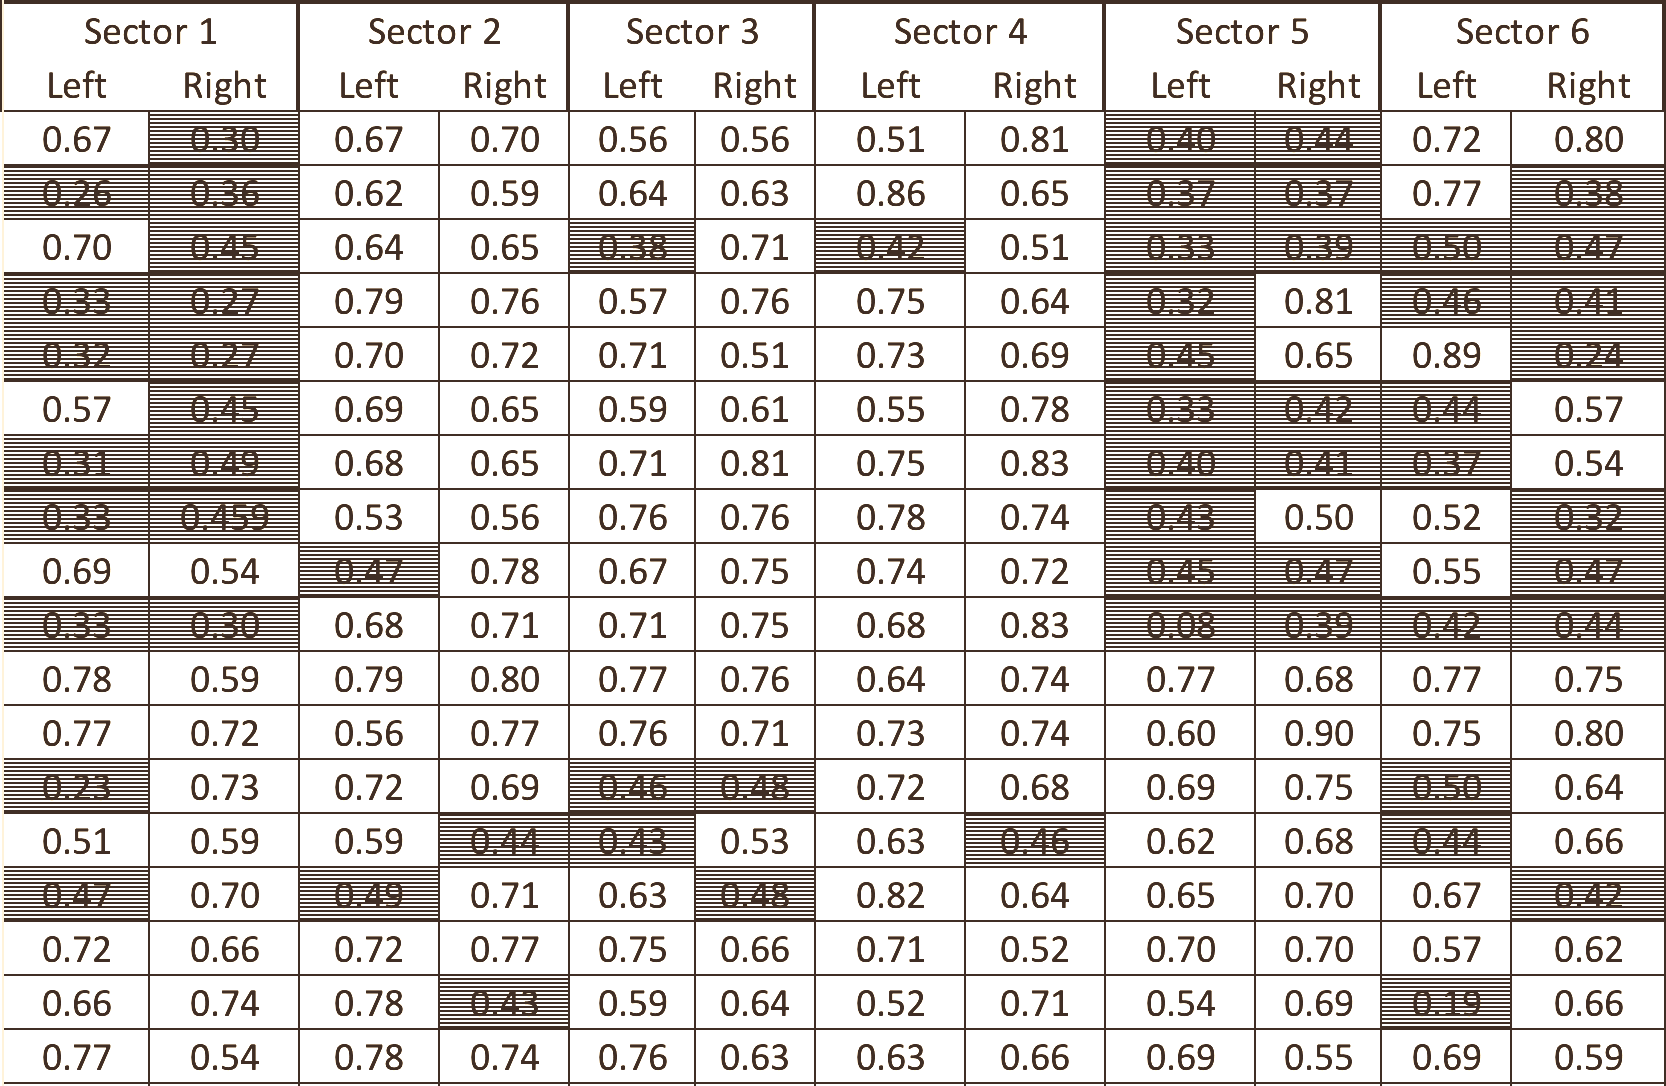
\includegraphics[width=0.95\columnwidth,keepaspectratio]{img/wcStatusBefore.png}
	\caption{Top: typical reflectivity of a "very poor" WC. The reflectivity is below 30\% for most of the wavelength between 200 and 400 nm. Bottom: the average reflectivity $r$ between 200 and 400 nm for
            all the WC. Legend: grey: ``very poor'' ($r < 30\%$); red: ``poor`` (30\% < $r < 50\%$); brown: ``so-so`` (50\% < $r < 70\%$); green: ``good`` (70\% < $r < 80\%$); yellow: ``excellent`` ( $r > 70\%$); }
	\label{fig:wcStatusBefore}
\end{figure}


\begin{figure}
	\centering
	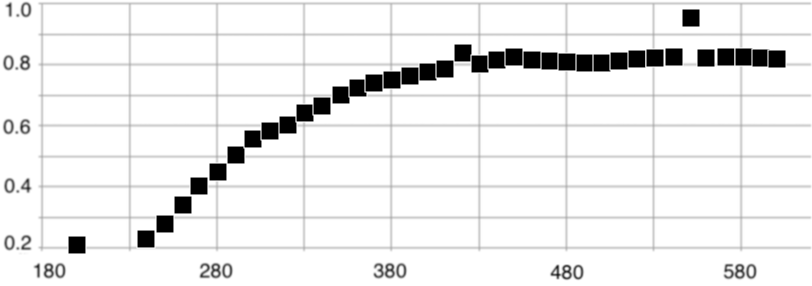
\includegraphics[width=1.0\columnwidth,keepaspectratio]{img/winstoConeSample1Reflectivity.png}
	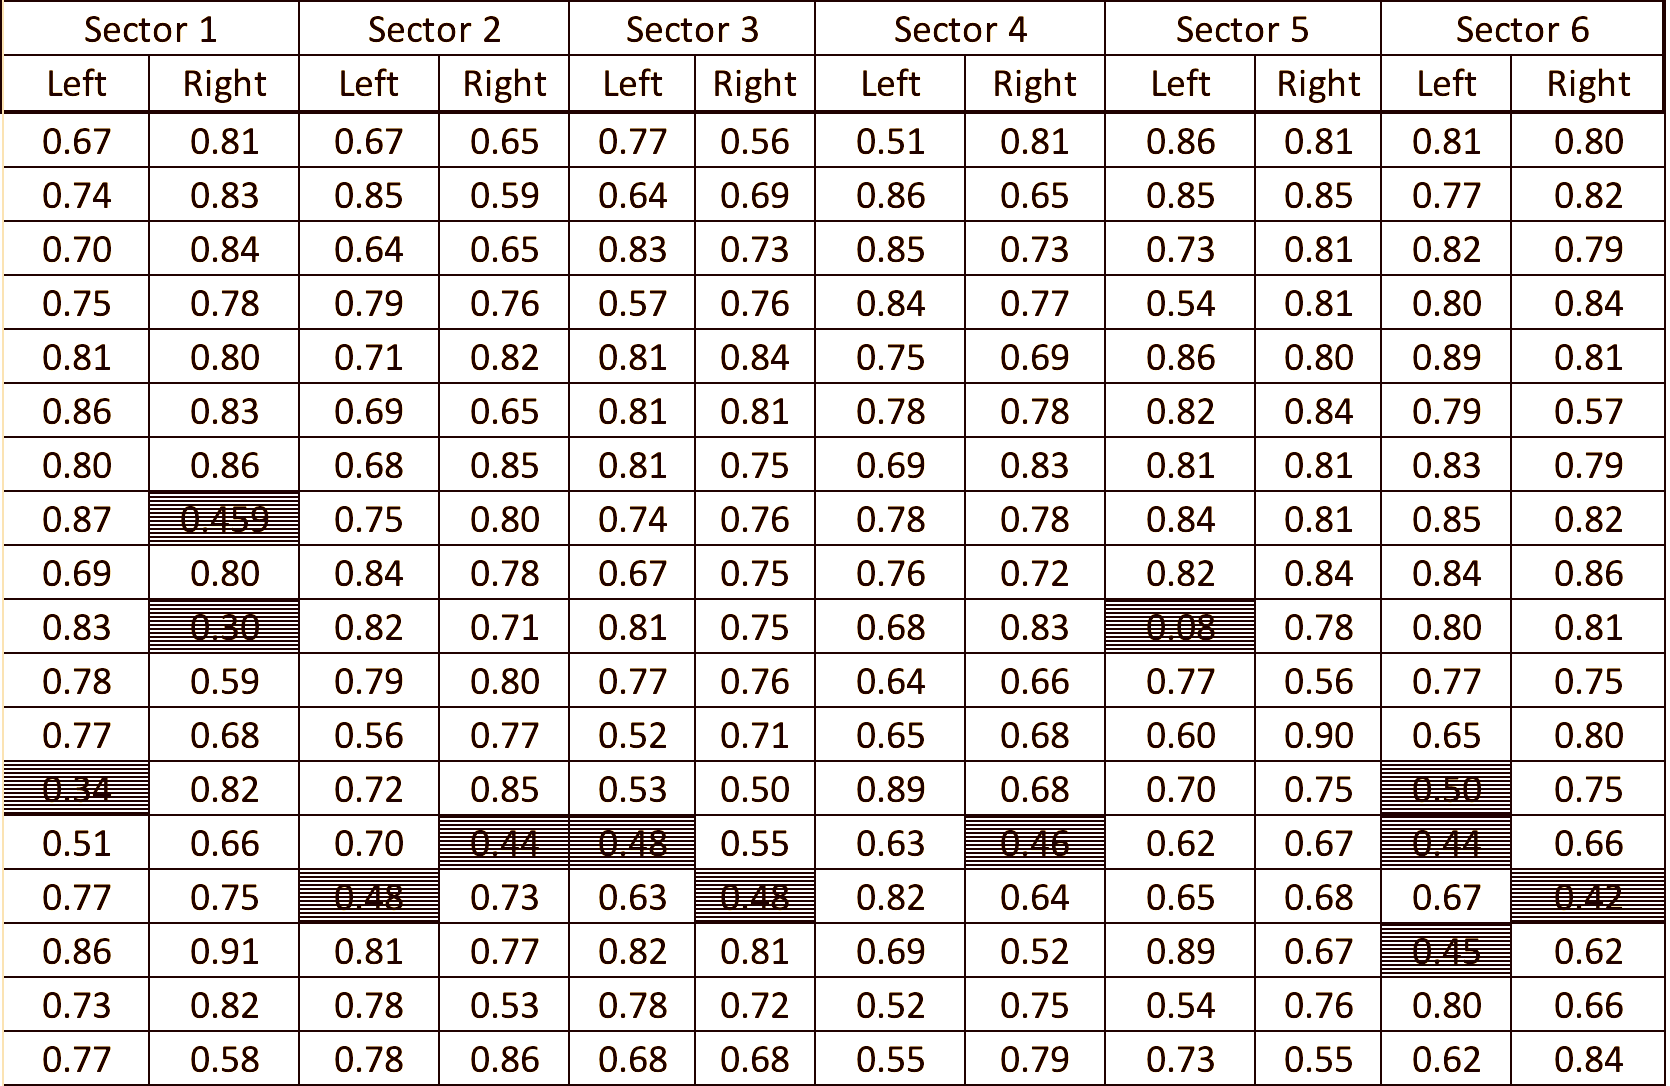
\includegraphics[width=1.0\columnwidth,keepaspectratio]{img/wcStatusAfter.png}
	\caption{Top: typical reflectivity of a "very poor" WC after refurbishment. The reflectivity quickly rise to $to\%$ at a wavelength of about 340 nm. Bottom: average WC reflectivity  $r$ between 200 and 400 nm for
				all the WC. This picture should be compared to \F{wcStatusAfter}. }
	\label{fig:wcStatusAfter}
\end{figure}



\subsection{Photo-multipliers surface coating}

The PMTs used in the LTCC are the photonis are the Photonis XP4500B \cite{Photonis:2007ta}.
Their borosilicate windows can be used to detect wavelengths as low as approximately
$300$ nm. However the Cherenkov light is inversely proportional to the wavelegth, see eq.~\ref{eq:cerenkov},
the $C_4F_{10}$ gas is transparent down to wavelengths of $180$ nm, and the mirrors and WCs reflectivities is non zero
even for wavelengths below $200$ nm: the limiting factor of enhanced QE in the UV region
is the transparency of the window material of the PMTs. UV-glass windows can detect photons down to
250 nm, and only quartz windows can efficiently detect light down to 180 nm. While quartz windows maximize the UV-sensitivity
of the PMT, and therefore the Cerenkov detector performance, they are difficult and expensive to produce.

A wavelength shifter (WLS) deposited on the face of a borosilicate or UV glass
PMT provides an effective alternative to boost the efficiency of a \u{C}erenkov
detector by converting UV photons with a wavelength below $300$ nm into two
isotropically emitted photons with longer wavelengths.



\begin{figure}
	\centering
	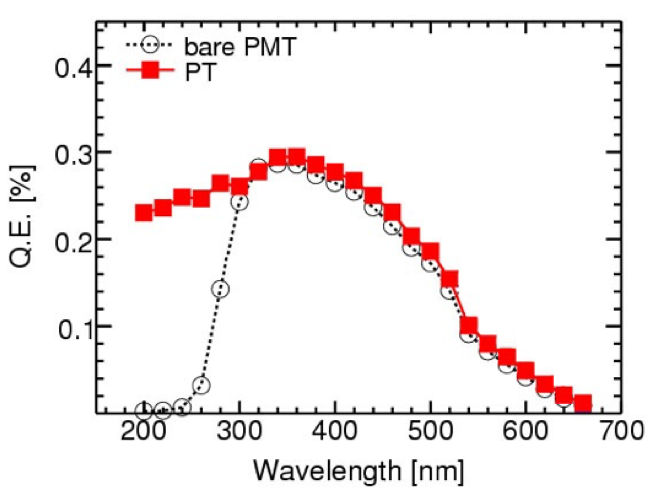
\includegraphics[width=1.0\columnwidth,keepaspectratio]{img/pmtQuantumEfficiencyGain.png}
	\caption{Average number of reflections calculated from simulations studies.}
	\label{fig:pmtQuantumEfficiencyGain}
\end{figure}

\begin{figure}
	\centering
	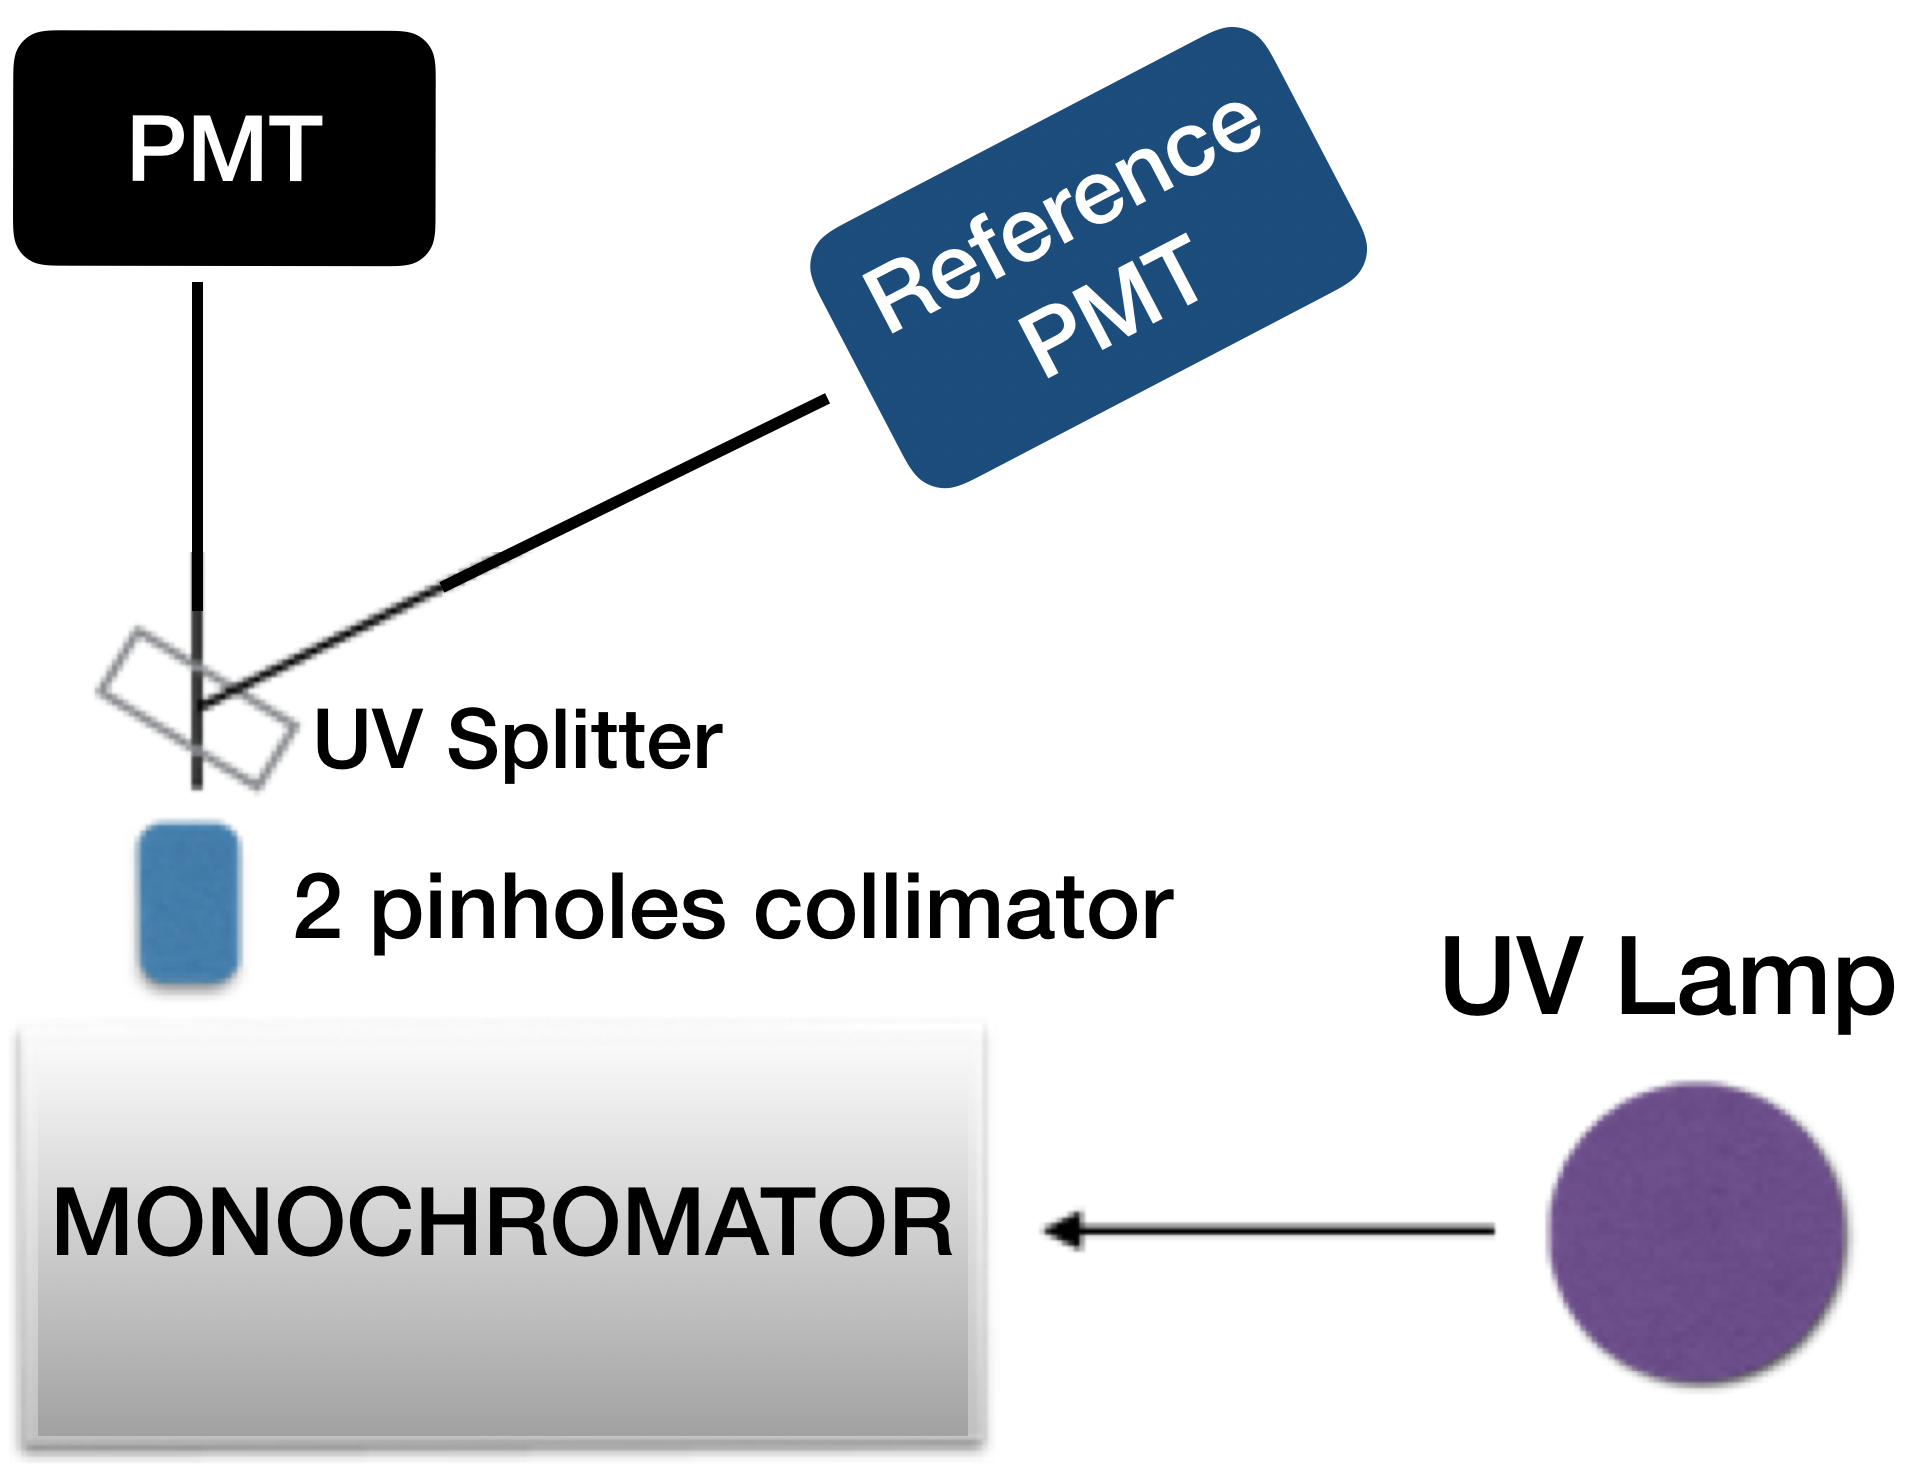
\includegraphics[width=1.0\columnwidth,keepaspectratio]{img/pmtTestingSetup.png}
	\caption{Average number of reflections calculated from simulations studies.}
	\label{fig:pmtTestingSetup}
\end{figure}





\subsection{Photo-multipliers Divider}

In the original readout electronics the LTCC single ouput from each PMT was amplified by a factor of 10
and then splitted in two to feed the ADC and TDC baords. This amplification and splitting was performed
by a dedicated electronic module. 

In 2002 a novel concept \cite{Popov:2003mj} was developed at Jefferson Lab to effectivly amplify a PMT signal by employing a dedicated circuit
to process the anode or dynode signal prior to sending it through a standard 50 $\omega$ line/cable.

The electronic addition to the PMT base provides an additional PMT signal boost while preserving
PMT fast pulse shape. It also improves rate capability. It significantly improves signal amplitude and
signal to noise ratio, which is especially important for low input light signals in cases such as Cherenkov counters.

The design was adapted to use the LTCC XP4500B base and a prototype, shown in \F{pmtWithDivider} was built to provide a x10
amplification and a splitted signal directly from the PMT base.


\begin{figure}
	\centering
	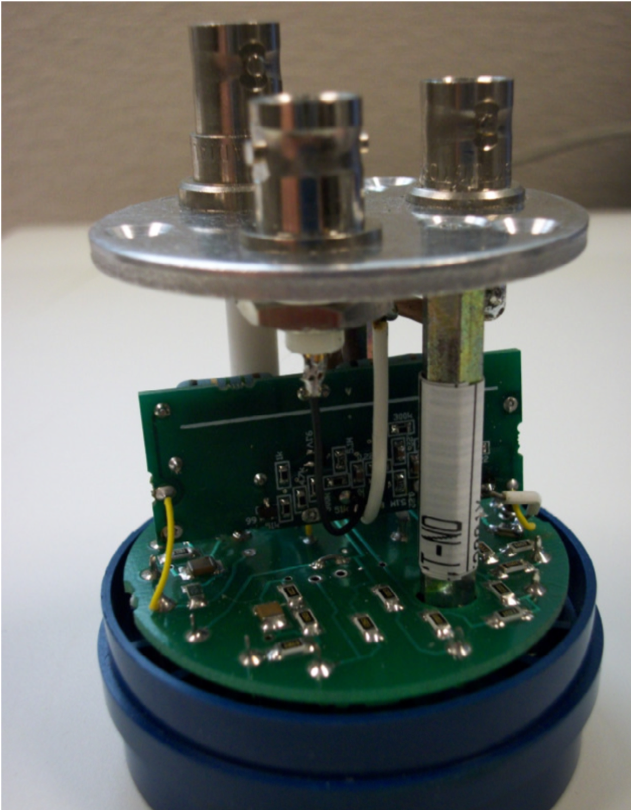
\includegraphics[width=0.95\columnwidth,keepaspectratio]{img/pmtWithDivider.png}
	\caption{The prototype module installed in the XP4500B PMT base. The bottom of the base has been modified to contain the HV
				BNC input and two output signals BNC. }
	\label{fig:pmtWithDivider}
\end{figure}

The following tests were performed successfully:
\begin{itemize}
	\item x10 amplification
	\item splitted signals identity
	\item signal to noise ratio comparison with non modified base
	\item FADC spectrum
\end{itemize}

In \F{dividerTests} (top) an empirical comparison of the two signals shows the similarity between the two output.
During testing of the modified PMT bases, the output has been processed by a Flash ADC electronic and acquired with a data
acquisition software using the PMT itself as trigger.
The corresponding SPE spectrum has been analyzed. The shape of the SPE signal is very similar to the original signal
coming from the external dedicated splitter and amplifier through the ADC electronics, see  \F{dividerTests} (bottom).

\begin{figure}
	\centering
	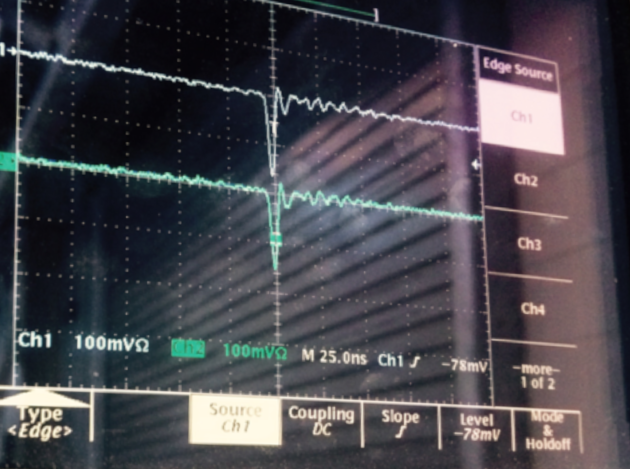
\includegraphics[width=0.87\columnwidth,keepaspectratio]{img/doubleSignal.png}
	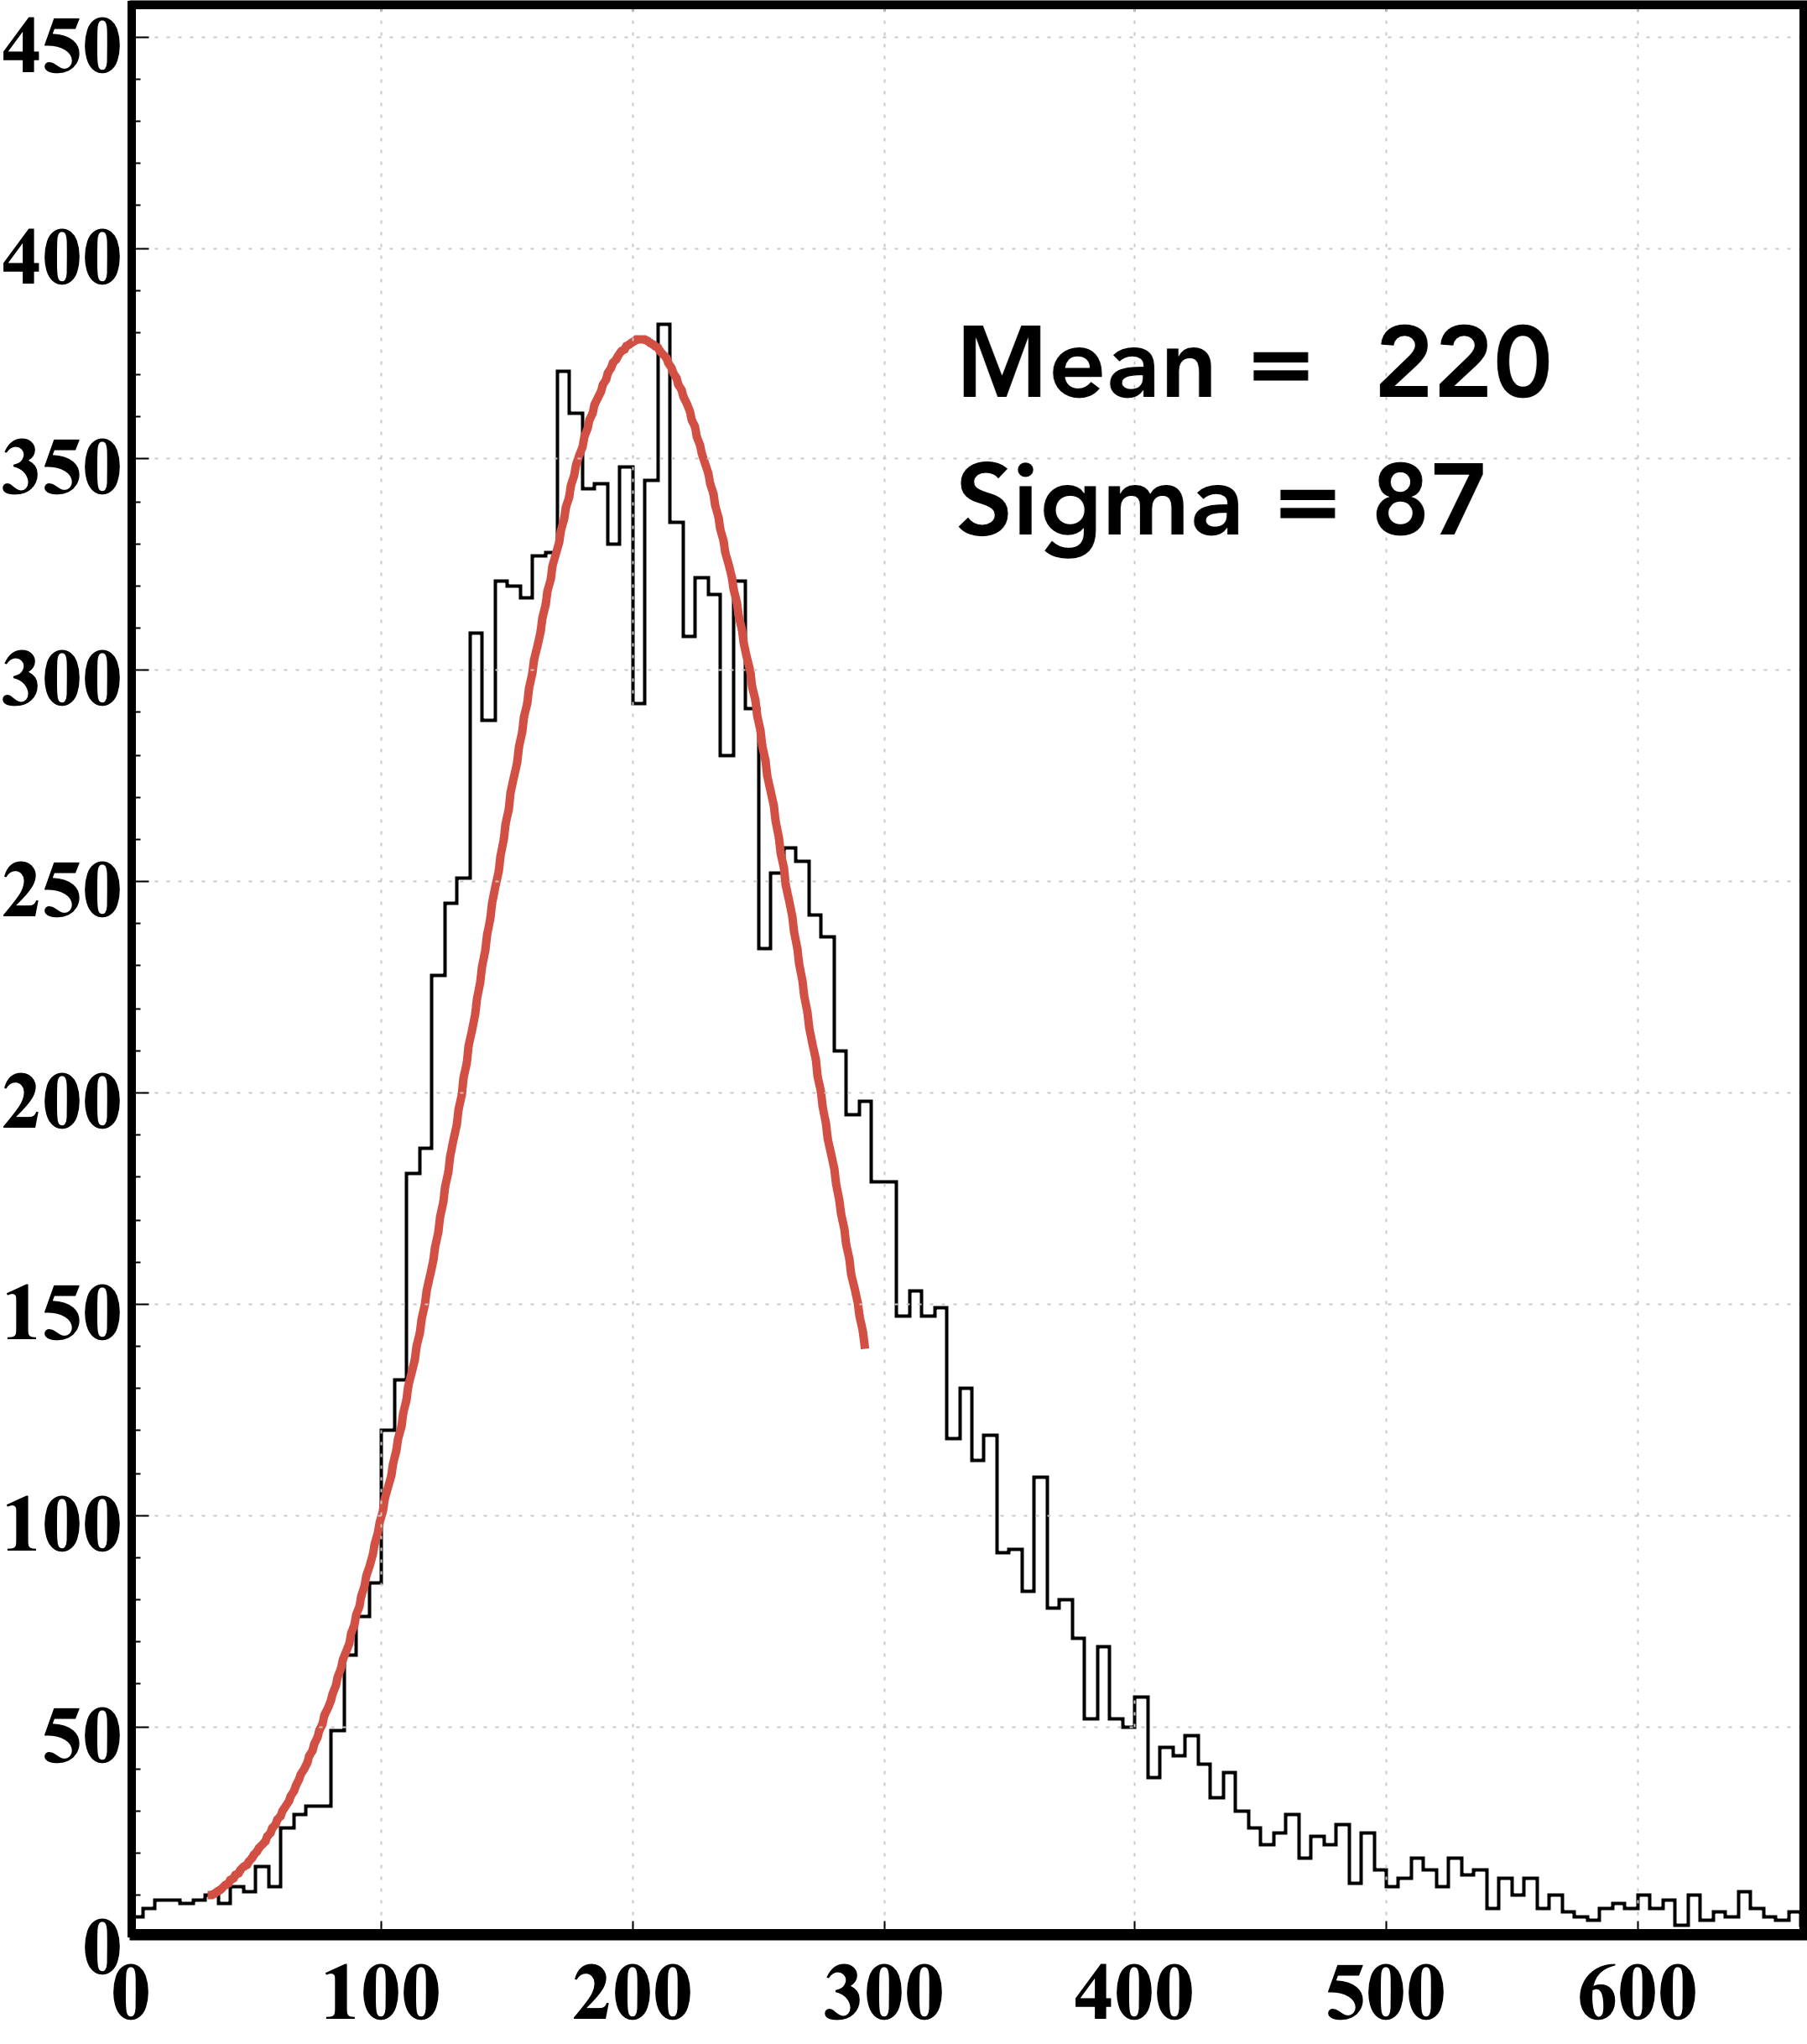
\includegraphics[width=0.97\columnwidth,keepaspectratio]{img/fadcOutput.png}
	\caption{Top: qualitetively comparison of the two outputs from the base modifications as seen on an oscilloscope.
				The analysis of the adc spectra histograms confirmed quantitevily that the signals are identical. Bottom:
				The single photo-electron ADC spectrum of one of the output compared with the PMT output in the original
            configuration of a dedicated external splitter and amplifier.
    }
	\label{fig:dividerTests}
\end{figure}

180 bases assembled at Jefferson Lab and installed on the PMT dividers. Both signals from all the modified bases were tested.
The response of the PMTs to the SPE resulted identical to the original output after it was amplified by a factor of 10, with one
clear advantage: the new bases allowed the PMTs to run at a HV average of 300 Volts less, see \F{pmtHVImprovement}.



\begin{figure}
	\centering
	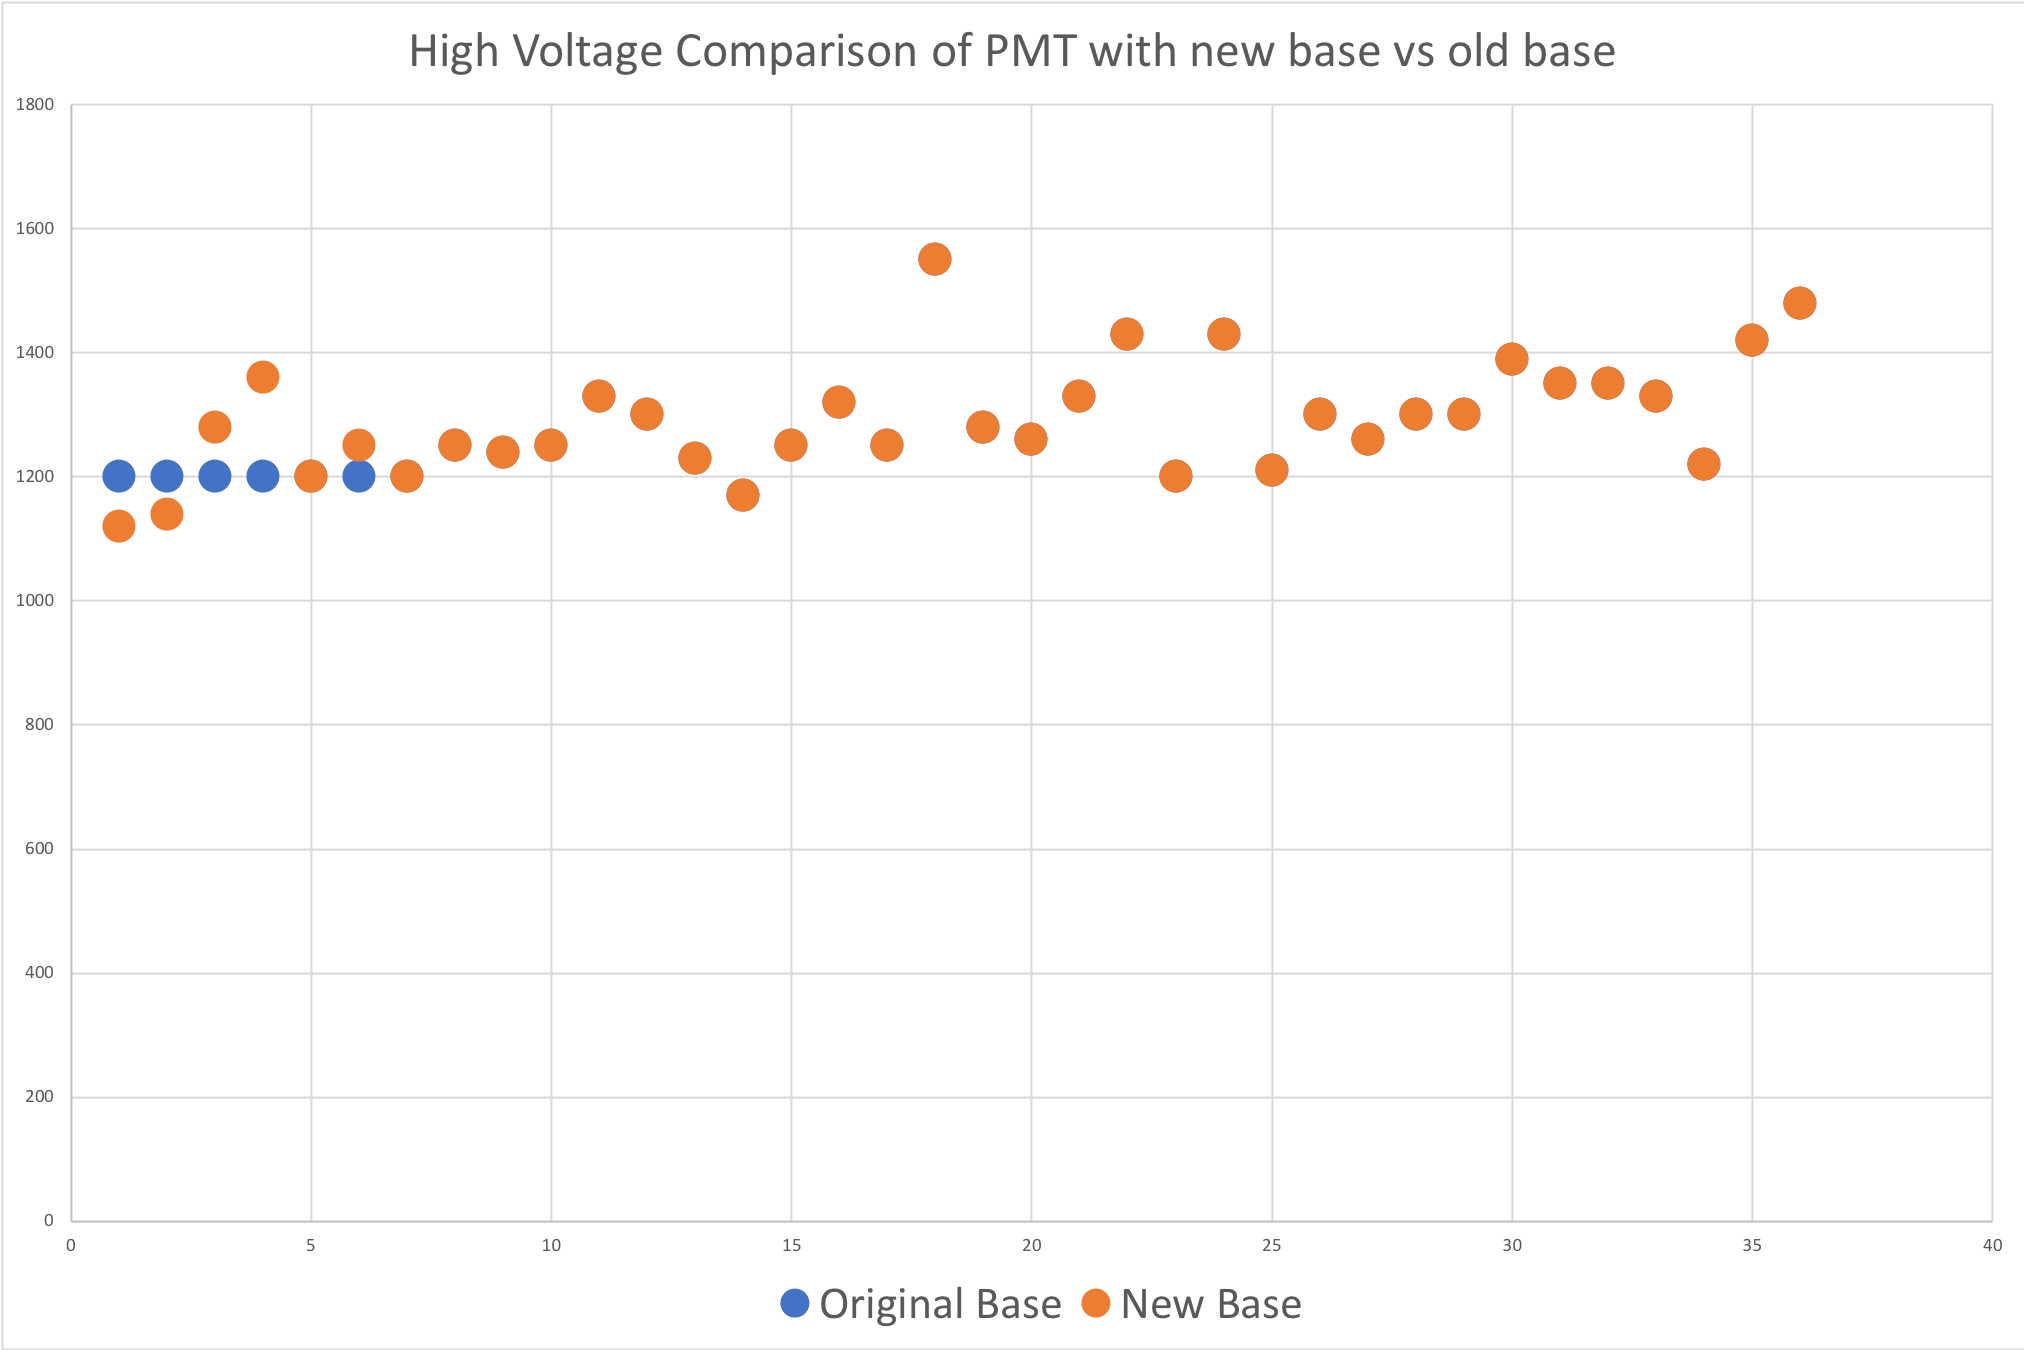
\includegraphics[width=0.95\columnwidth,keepaspectratio]{img/pmtHVImprovement.png}
	\caption{The PMTs with the modified bases could produce the same response function of the original base but at about 300 HV less voltage.}
	\label{fig:pmtHVImprovement}
\end{figure}


\subsection{The LTCC Windows}

The LTCC windows that cover the upstream and downstream open frame of the box are a composite of
Tedlar/Mylar/Tedlar, see \F{windowDesign}. Two layers of the Tedlar film provide reliable light tightness
even if they have some defects such as wrinkles and small pinholes through, while the Mylar portion
adds the material strength necessary to withstand gas differential pressure and increase wear resistance
and reliability. This design, easy to handle and apply to the module,
simplified the replacement of the old composite window.

\begin{figure}[!ht]
	\centering
	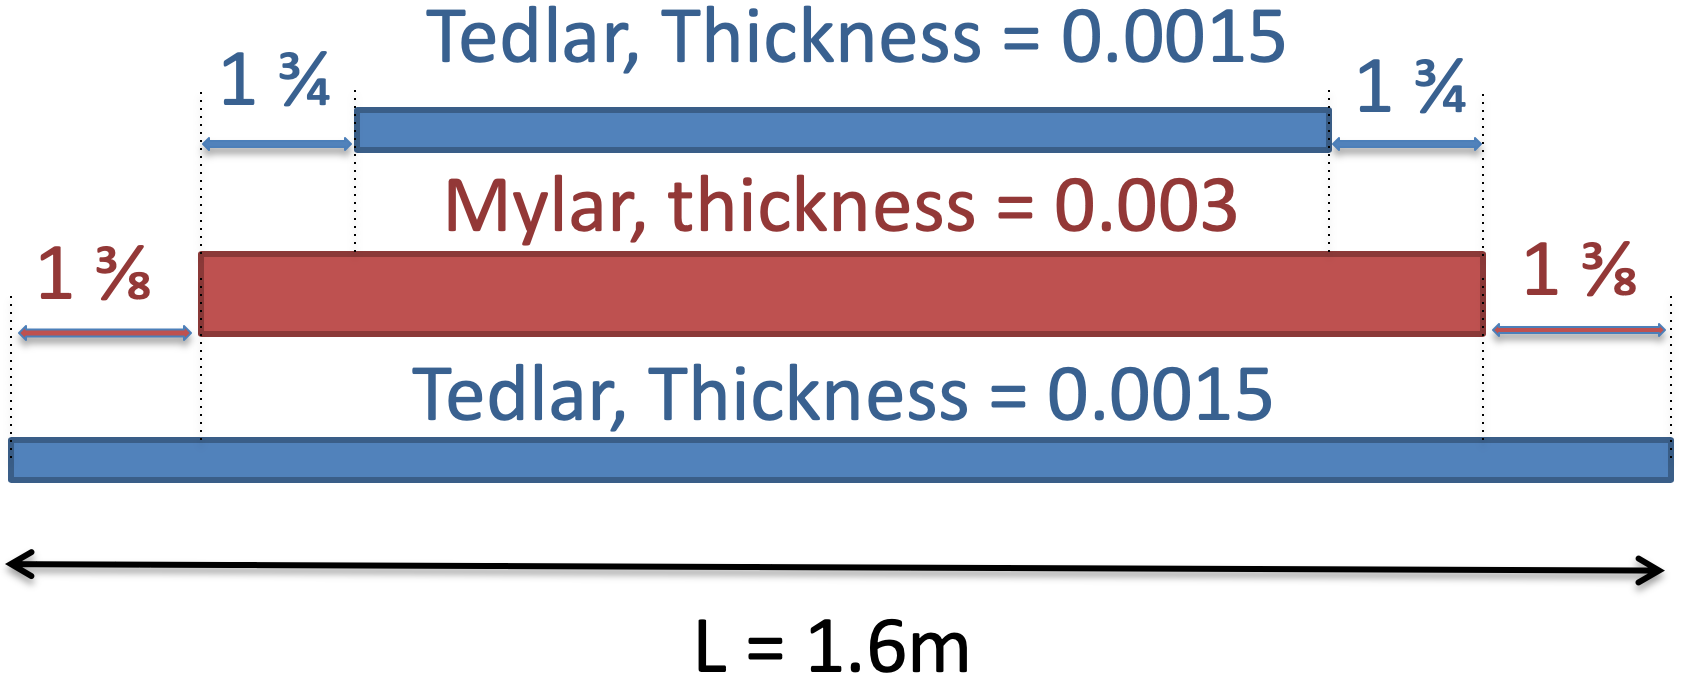
\includegraphics[width=0.98\columnwidth, keepaspectratio]{img/windowDesign.png}
	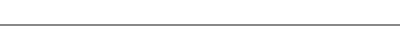
\includegraphics[width=0.98\columnwidth, height=0.1\columnwidth]{img/blank.png}
	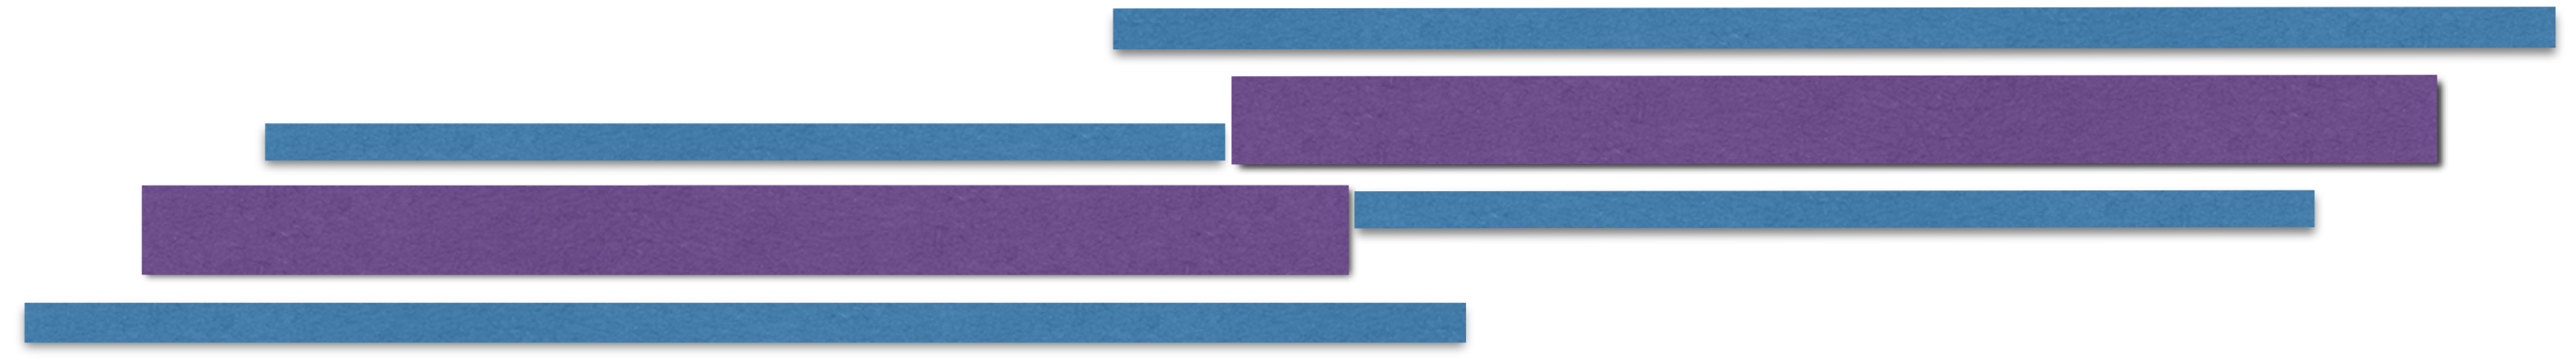
\includegraphics[width=0.98\columnwidth, keepaspectratio]{img/windowSeaming.png}
	\caption{Top: the design of the LTCC Tedlar/Mylar/Tedlar window sandwich. The pyramid design allowed for the
          seaming shown at the bottom. Bottom: the seaming design involves gluing Mylar to Mylar to ensure that the window
          stress is transmitted entirely to the Mylar.}
	\label{fig:windowDesign}
\end{figure}


The window was fabricated in two steps:

\begin{enumerate}
	\item lamination of 1.6~m wide Tedlar/Mylar/Tedlar rolls
	\item seaming of the laminated strips into a 4.8~m $\times$ 4.8~m window
\end{enumerate}

The lamination of the composite material, with dimensions outlined in \F{windowDesign} (top), was performed at
Madico~\cite{madico}, where a sheet 400~m long was produced.

At Jefferson Lab rectangles were cut out of the laminated sheet, each 1.6~m wide and 4.8~m long. To form a final
4.8~m $\times$ 4.8~m single LTCC window, three of the rectangles were seamed together using G/Flex 655 epoxy.
The seam was load tested to withstand a pressure 10 times higher than that expected from the C$_4$F$_{10}$ gas flow and gas weight.

\subsubsection{Window Installation and Gas Leak Tests}

The installation of the window onto the box was achieved through gluing the window on the box sides using G/Flex 655
epoxy. The width of the window attached with glue was 12~cm, to provide sufficient gluing area. A photograph of the
downstream window after installation is shown in \F{downstreamWindow}.

\begin{figure}
	\centering
	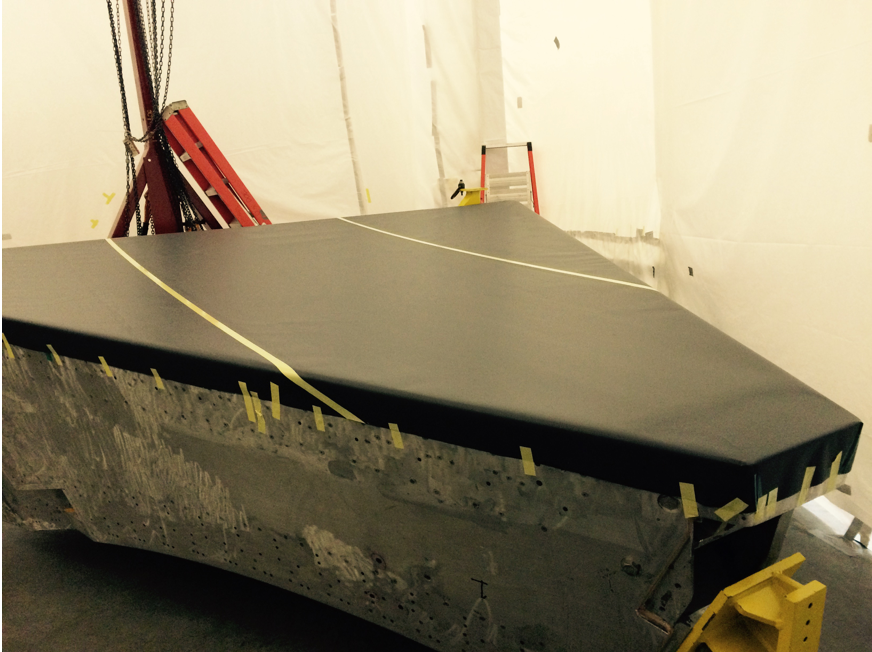
\includegraphics[width=1.0\columnwidth,keepaspectratio]{img/downstreamWindow.png}
	\caption{The downstream window of one LTCC sector during curing of the epoxy. The yellow strips protect the
          window seaming.}
	\label{fig:downstreamWindow}
\end{figure}

After curing of both the upstream and downstream windows, the LTCC box was filled with nitrogen gas to a
positive differential pressure of
2~in of water. Freon gas was pumped into the box and leaks were detected using a refrigerant leak detector. After the
leaks were sealed, the box was pressurized for a 48 hour period to test the overall box gas tightness. This procedure
was repeated after every movement of the LTCC boxes, as small shifts of the frame walls had the potential to introduce
additional leaks due to the large surface area of the detector.


